

\section{The Human Imitator: A Scalable Testbed}
\label{sec:imitator}

To rigorously evaluate our agentic framework presented in \Cref{sec:framework}, we must confront a fundamental methodological challenge: the scarcity of realistic testbeds. Standard inventory benchmarks rely on static, structured parameters, failing to capture the ambiguity, inconsistency, and bounded rationality that define real-world decision-making. Conversely, human-subject experiments, while ecologically valid, are costly, unscalable, and difficult to reproduce.

We bridge this gap by developing the \emph{Human Imitator}—an LLM fine-tuned to function as a ``digital twin'' of a retail manager. Unlike a standard LLM, which strives for helpfulness and precision, our imitator is explicitly trained to reproduce the idiosyncrasies of human behavior: providing rough estimates, using informal language, and occasionally omitting critical details. This allows us to stress-test our system against realistic ``human noise'' at scale.

\subsection{Data Collection: Capturing Managerial Dialogue}

We constructed a specialized corpus of inventory management dialogues through a controlled study. We deployed an online interface where participants played the role of a store manager interacting with a generic ``Base Model'' consultant. The Base Model was prompted to elicit specific operational parameters—including demand patterns, perishability, holding costs, and lead times—while the participants were instructed to describe their business scenario using natural language.

This process yielded a dataset of prompt–response pairs, $\mathcal{D} = \{ (x^{(i)}, y^{(i)} \}_{i=1}^N$, where $x^{(i)}$ represents the system's inquiry (e.g., \emph{``How long do items stay fresh?''}) and $y^{(i)}$ represents the human's verbatim response (e.g., \emph{``maybe 3 days max''}). 

In total, $66$ participants generated $N = 1,184$ high-quality conversational turns. This dataset captures a diverse range of linguistic styles, from precise specifications to vague, heuristic-driven descriptions. Detailed screenshots of the interface and example transcripts of the collected dialogues are provided in \Cref{sec:SFT}.

\subsection{Supervised Fine-Tuning (SFT)}

To instill human-like behavioral patterns into the model, we performed Supervised Fine-Tuning (SFT) on the \emph{Qwen2.5-7B} foundation model. We treat the imitator as a policy $\policytheta$ parameterized by weights $\paratheta$. The training objective is to maximize the likelihood of generating the empirically observed human response $\response$ given the context $\prompt$:
\[
\max_\theta \quad \sum_{(\prompt^{(i)}, \response^{(i)}) \in \Data} \log \policytheta \big(\response^{(i)} \bigm| \prompt^{(i)} \big).
\]
This objective forces the model to align its probability distribution with human behavior, effectively teaching it to ``unlearn'' robotic precision and adopt the persona of a boundedly rational manager.

Since our goal is \emph{imitation}—creating a faithful proxy that reproduces the specific distribution of our target population—we train on the full dataset to maximize behavioral coverage. Training was conducted using Low-Rank Adaptation (LoRA) on a single NVIDIA L4 GPU (24GB). The optimization converged rapidly over 3 epochs (524 minutes), with the loss function reducing from $1.9234$ to $0.3473$, indicating that the foundation model successfully adapted to the domain-specific linguistic patterns. See \Cref{sec:SFTtraining} for experimental details. 

\subsection{Empirical Validation: Quantifying Behavioral Alignment}

Does the fine-tuned model truly resemble a human manager? We monitor the model's fidelity across four metrics that measure alignment at distinct linguistic levels: \emph{fluency}, \emph{structure}, \emph{token usage}, and \emph{sentence meaning}. The training trajectory is visualized in \Cref{fig:SFT_eval}, with numerical results detailed in \Cref{tab:sft-eval}.

\begin{figure}[!ht]
    \centering
    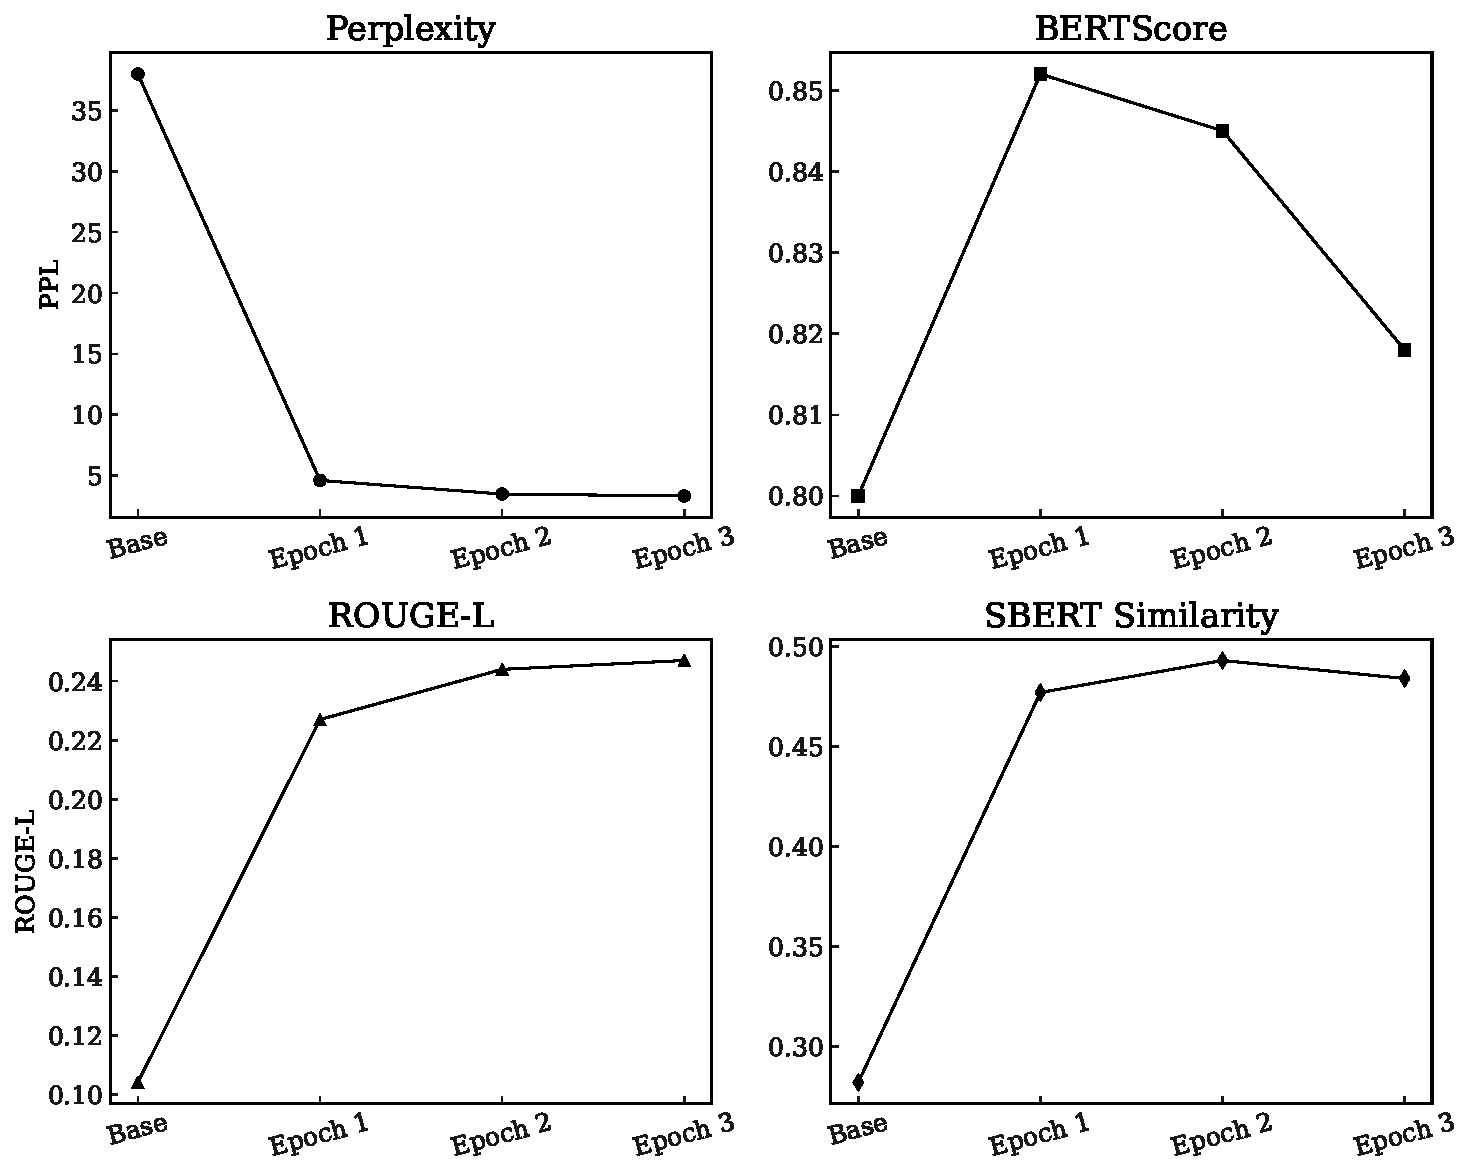
\includegraphics[width = 0.75 \linewidth]{fig/SFT_eval} 
    \caption{\textbf{SFT Evaluation Trajectory.} The curves illustrate the rapid convergence of the Human Imitator. \\
    The drop in Perplexity and the simultaneous rise in semantic similarity metrics (BERTScore, ROUGE-L and SBERT) indicate successful domain adaptation.}
    \label{fig:SFT_eval}
\end{figure}

\begin{table}[ht]
    \centering
    \renewcommand{\arraystretch}{1.2}
    \begin{tabular}{l S[table-format=2.3] S[table-format=1.3] S[table-format=1.3] S[table-format=1.3]}
        \toprule
        \textbf{Training Stage} & \textbf{PPL} $\downarrow$ & \textbf{BERTScore} $\uparrow$ & \textbf{ROUGE-L} $\uparrow$ & \textbf{SBERT} $\uparrow$ \\
        \midrule
        Epoch 0 (Base) & 37.991 & 0.800 & 0.104 & 0.282 \\
        Epoch 1        &  4.615 & \textbf{0.852} & 0.227 & 0.477 \\
        Epoch 2        &  3.487 & 0.845 & 0.244 & \textbf{0.493} \\
        Epoch 3        &  \textbf{3.334} & 0.818 & \textbf{0.247} & 0.484 \\
        \bottomrule
    \end{tabular}
    \caption{\textbf{Validation of the Human Imitator.} We track four metrics across training epochs. \emph{PPL} measures predictive certainty (lower is better). \emph{BERTScore} measures token-level embedding similarity. \emph{ROUGE-L} measures structural Longest Common Subsequence (LCS) overlap. \emph{SBERT} measures sentence-level semantic alignment.}
    \label{tab:sft-eval}
\end{table}

\paragraph{Drastic Reduction in Perplexity (Domain Adaptation):}
The most critical indicator of success is Perplexity (PPL), which measures the model's predictive uncertainty regarding the next token. As shown in \Cref{tab:sft-eval}, the PPL drops precipitously from $37.99$ (Base~Model) to $3.33$ (Epoch~3). This order-of-magnitude improvement confirms that the model, which initially spoke like a generic assistant, has successfully adopted the specific jargon, hesitation, and vernacular of human input.

\paragraph{Semantic and Structural Convergence:}
To ensure the model captures the \emph{intent} and \emph{style} of the managers, we examine similarity metrics at three levels of abstraction:
\begin{itemize}
    \item \emph{BERTScore (Token-Level Embedding Similarity):} BERTScore computes the cosine similarity between contextual embeddings of individual tokens. A high score (e.g. $0.85$) confirms that the model is selecting the correct \emph{vocabulary} within context, ensuring granular alignment with the specific terminology used by inventory managers.
    \item \emph{ROUGE-L (Structural Similarity):} ROUGE-L measures the Longest Common Subsequence (LCS) between the generated and reference text. The significant rise (from 0.104 to 0.247) indicates that the imitator is replicating the \emph{syntactic structure} of the participants—mimicking the sentence fragments, brevity, and informal phrasing typical of the domain.
    \item \emph{SBERT (Sentence-Level Semantic Similarity):} SBERT computes embeddings for the entire sentence. The doubling of this metric (from 0.282 to 0.493) confirms that the model is capturing the \emph{holistic semantic intent} of the human response, ensuring that the generated ``noise'' preserves the underlying meaning of the parameter description.
\end{itemize}

Based on these results, we selected the checkpoint at \textbf{Epoch~2} for our experiments. While Epoch~3 achieves a marginally lower perplexity, we observe a degradation in semantic alignment, evidenced by the sharp drop in BERTScore (from 0.845 to 0.818). In contrast, Epoch~2 achieves the highest SBERT similarity ($0.493$) while maintaining a high BERTScore. This suggests that Epoch~2 offers the optimal trade-off: it preserves the highest semantic fidelity to human intent without overfitting to the specific lexical patterns of the training data. The result is a robust, scalable proxy that authentically simulates the ``last mile'' friction of inventory management.

